\documentclass[10pt, aspectratio=169]{beamer}
\usetheme{metropolis}
\metroset{block=fill}
\setbeamercolor{block title}{bg=teal!20, fg=black}
\setbeamercolor{block body}{bg=teal!5}
\usepackage{booktabs}
\usepackage{graphicx}
\usepackage{xcolor}
\usepackage{colortbl}
\usepackage{amsmath}
\usepackage{hyperref}
\usepackage{appendixnumberbeamer}

\title{How Does Geometric Bias Shape the Denoising Trajectory\\in Flow-Based Protein Structure Generation?}
\author{Shreyas Ravishankar}
\institute{University of Cambridge}
\date{}

\begin{document}

% ============================================================
\begin{frame}[plain]
\titlepage
\end{frame}

% ============================================================
\begin{frame}{Proteina: Geometry via Additive Pair Bias}

\textbf{Flow matching:} SDE from noise to backbone \quad $t = 0 \xrightarrow{\text{100 SDE steps}} t = 1$

\medskip
\textbf{Every attention layer computes:} \quad $A = \mathrm{softmax}(C + B)$

\medskip
\begin{itemize}\setlength\itemsep{0.6em}
    \item $C = QK^\top\!/\sqrt{d}$, the learned content score
    \item $B$ = geometric pair bias, constructed from binned pairwise C$\alpha$ distances and sequence separation.
    Recomputed every denoising step from the current noisy structure $\mathbf{x}_t$:
    uninformative at $t{=}0$ (noise), encodes near-final backbone at $t{=}1$.
\end{itemize}

\vfill

\begin{block}{Two questions}
\emph{When} does $B$ become causally essential during generation?\\
\emph{Where} in the network does it act?
\end{block}

\end{frame}

% ============================================================
\begin{frame}{Methods: Four Lenses, Four Model Scales}
\begin{columns}[T]
\begin{column}{0.45\textwidth}

\textbf{Analysis lenses:}
\begin{enumerate}\setlength\itemsep{0.4em}
    \item \textbf{Descriptive} --- how large is $B$ vs $C$?
    \item \textbf{Causal} --- when/where must $B$ be present?
    \item \textbf{Functional} --- which encodes contacts better?
    \item \textbf{Representational} --- where does 3D structure emerge?
\end{enumerate}

\end{column}
\begin{column}{0.50\textwidth}

\textbf{Four model variants:}
\smallskip

{\small
\begin{tabular}{lccc}
    \toprule
    Model & Layers & Params & Triangle \\
    \midrule
    60M no-tri & 12 & 60M & No \\
    200M no-tri & 15 & 200M & No \\
    200M tri & 15 & 200M & Yes \\
    400M tri & 18 & 400M & Yes \\
    \bottomrule
\end{tabular}}

\end{column}
\end{columns}
\end{frame}

% ============================================================
\begin{frame}{Descriptive: Geometry Dominance in Peak Layers}

\begin{figure}
    \centering
    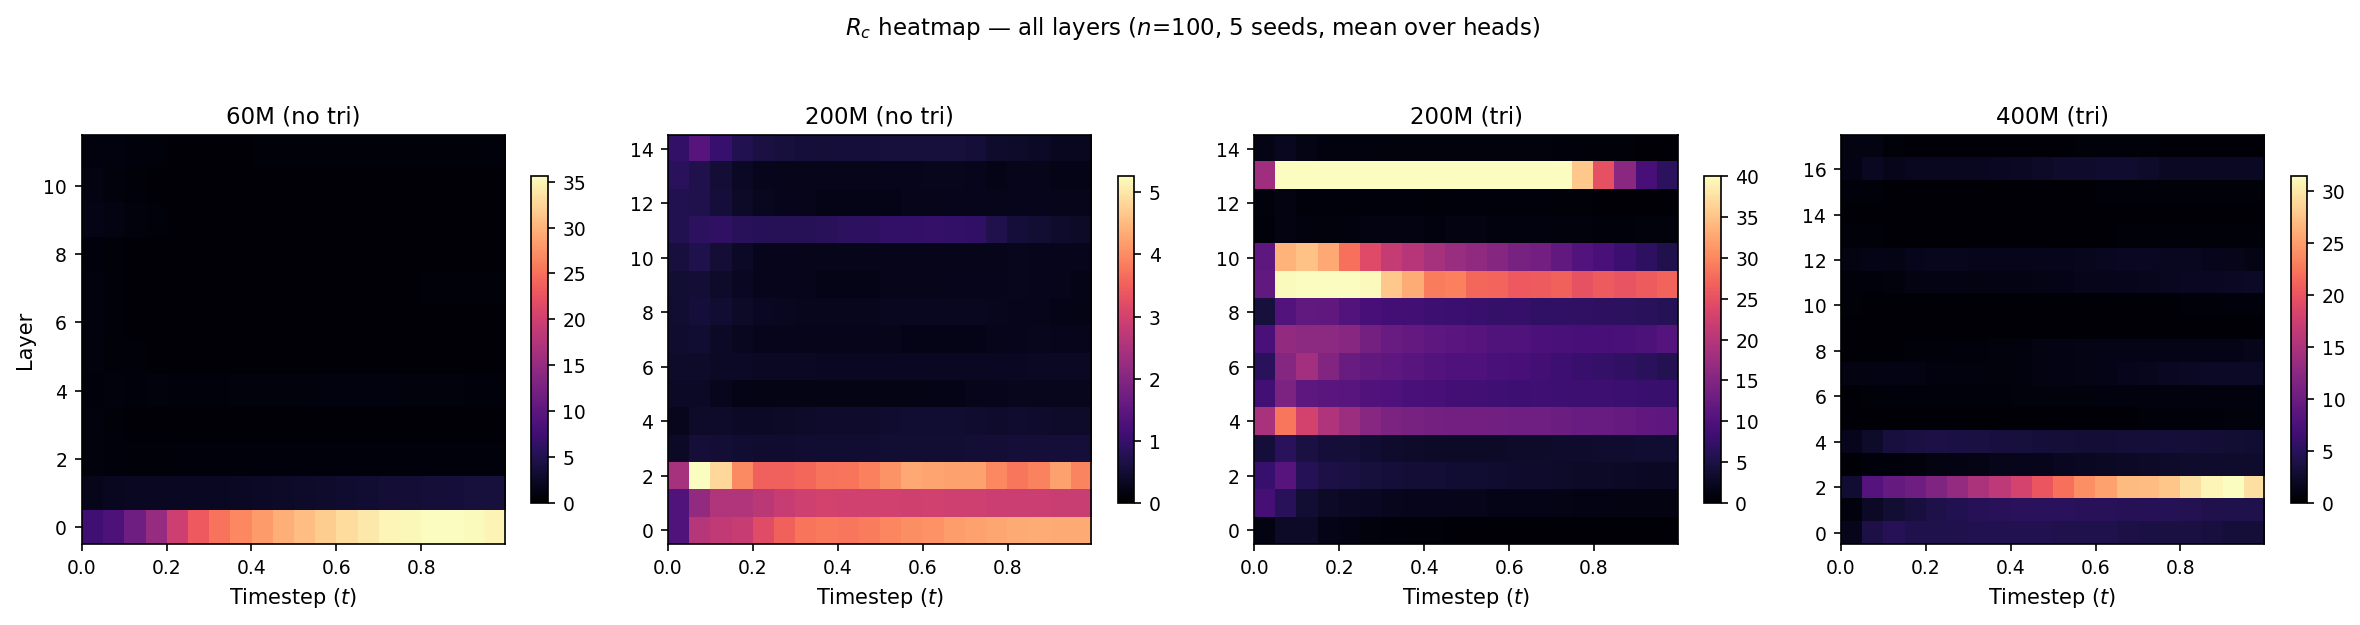
\includegraphics[width=0.92\textwidth]{figures/fig1b-Rc-heatmaps.png}
\end{figure}

\smallskip
Every model concentrates geometry dominance in a few peak layers, but the location is model-specific.

\medskip
\textbf{But:} descriptive magnitude $\neq$ causal importance --- the peak-$R_c$ layer is \emph{not} the causally critical layer.
\end{frame}

% ============================================================
\begin{frame}{Causal: The Late Phase Matters; the Early Phase Does Not}

\centering
{\footnotesize\renewcommand{\arraystretch}{1.1}
\begin{tabular}{lcccccccc}
    \toprule
    & \multicolumn{2}{c}{\textbf{60M no-tri}} & \multicolumn{2}{c}{\textbf{200M no-tri}} & \multicolumn{2}{c}{\textbf{200M tri}} & \multicolumn{2}{c}{\textbf{400M tri}} \\
    \cmidrule(lr){2-3} \cmidrule(lr){4-5} \cmidrule(lr){6-7} \cmidrule(lr){8-9}
    & $R_g$ & Cl & $R_g$ & Cl & $R_g$ & Cl & $R_g$ & Cl \\
    \midrule
    \textcolor{red!70!black}{Early-only $B$ ($t{\leq}0.5$)} & \textcolor{red!70!black}{0.12} & \textcolor{red!70!black}{3532} & \textcolor{red!70!black}{0.14} & \textcolor{red!70!black}{2967} & \textcolor{red!70!black}{0.07} & \textcolor{red!70!black}{4702} & \textcolor{red!70!black}{0.11} & \textcolor{red!70!black}{4021} \\
    \textcolor{teal!80!black}{Late-only $B$ ($t{>}0.5$)} & \textcolor{teal!80!black}{1.19} & \textcolor{teal!80!black}{0} & \textcolor{teal!80!black}{1.19} & \textcolor{teal!80!black}{4} & \textcolor{teal!80!black}{1.12} & \textcolor{teal!80!black}{2} & \textcolor{teal!80!black}{1.17} & \textcolor{teal!80!black}{1} \\
    \bottomrule
\end{tabular}}

\medskip
\begin{figure}
    \centering
    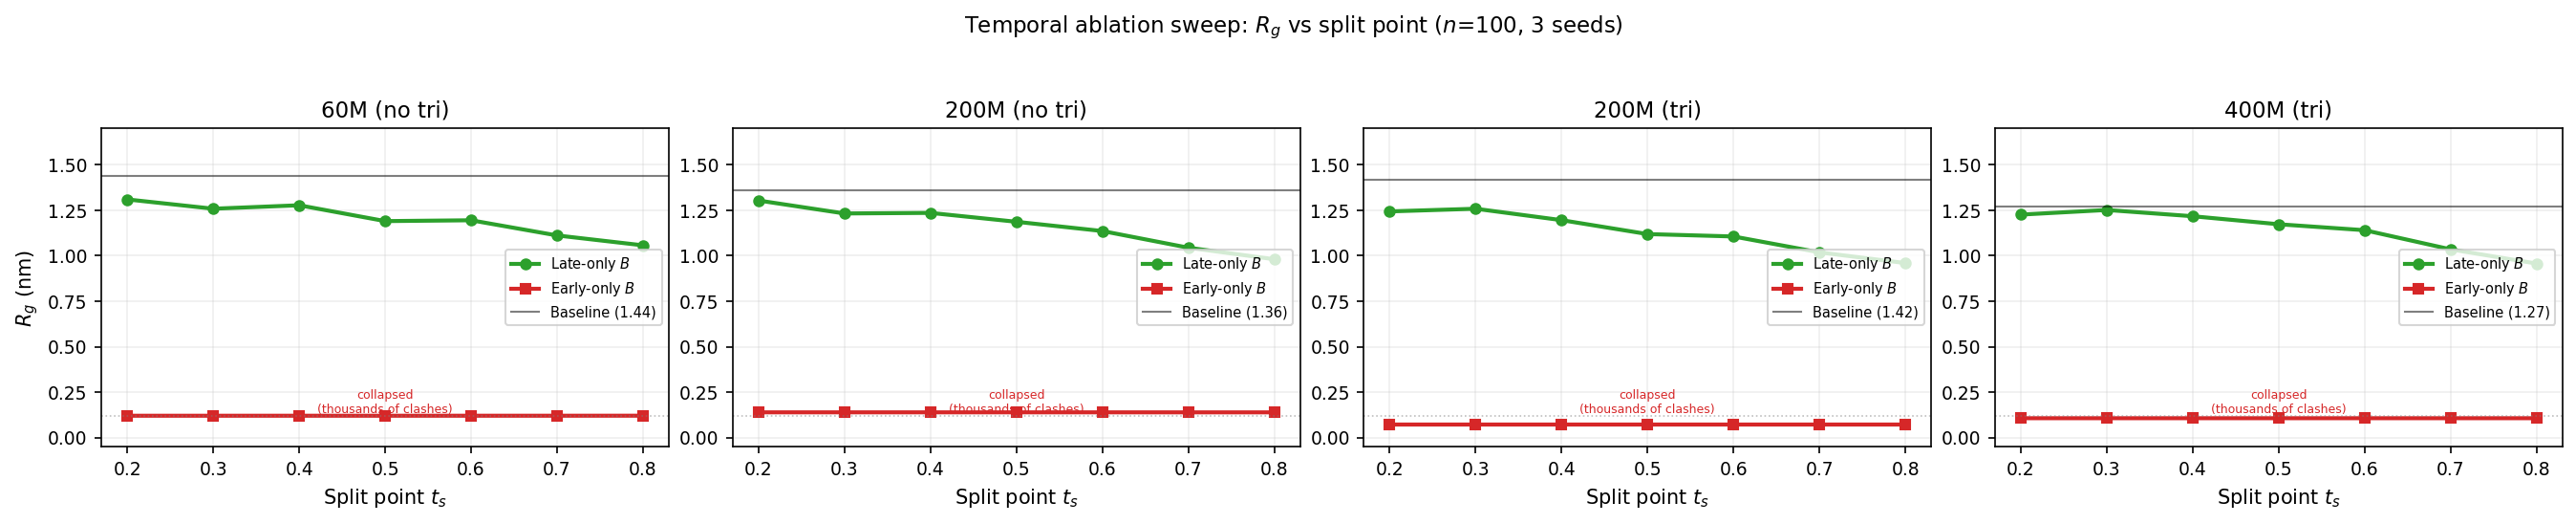
\includegraphics[width=0.85\textwidth]{figures/fig4-temporal-sweep.png}
\end{figure}

\end{frame}

% ============================================================
\begin{frame}{Causal: The Model Has No Memory of Early $B$}

\textbf{Gap experiment:} $B$ on $[0, 0.3]$, off $(0.3, 0.7)$, restored $[0.7, 1]$

\medskip
{\small
\begin{tabular}{lcccccccc}
    \toprule
    & \multicolumn{2}{c}{\textbf{60M no-tri}} & \multicolumn{2}{c}{\textbf{200M no-tri}} & \multicolumn{2}{c}{\textbf{200M tri}} & \multicolumn{2}{c}{\textbf{400M tri}} \\
    \cmidrule(lr){2-3} \cmidrule(lr){4-5} \cmidrule(lr){6-7} \cmidrule(lr){8-9}
    Condition & $R_g$ & Cl & $R_g$ & Cl & $R_g$ & Cl & $R_g$ & Cl \\
    \midrule
    Baseline & 1.44 & 0 & 1.36 & 0 & 1.42 & 0 & 1.27 & 1 \\
    \rowcolor{teal!10} Gap (on--off--on) & 1.10 & 0 & 1.04 & 3 & 1.01 & 3 & 1.05 & 1 \\
    \rowcolor{teal!10} Late-only ($t{>}0.7$) & 1.11 & 0 & 1.04 & 3 & 1.02 & 2 & 1.04 & 1 \\
    \bottomrule
\end{tabular}}

\bigskip
Gap $\approx$ Late-only within 0.02\,nm across all four models.
$\Rightarrow$ \textbf{Geometric guidance is memoryless:} the trajectory forgets both the presence and absence of early $B$.
\end{frame}

% ============================================================
\begin{frame}{Causal: Architecture Inverts Which Layers Are Critical}

\centering
{\small
\begin{tabular}{lcccc}
    \toprule
    Condition & 60M no-tri & 200M no-tri & 200M tri & 400M tri \\
    \midrule
    Baseline $R_g$ & 1.44 & 1.36 & 1.42 & 1.27 \\
    \midrule
    \textcolor{red!70!black}{Deep-only $B$} & \textcolor{red!70!black}{0.41} & \textcolor{red!70!black}{0.57} & 0.90 & 0.82 \\
    Shallow-only $B$ & 0.60 & 0.63 & \textcolor{red!70!black}{0.05} & \textcolor{red!70!black}{0.12} \\
    \midrule
    Peak-$R_c$ only & 0.81 & 1.28 & 1.17 & 1.13 \\
    \bottomrule
\end{tabular}}

\smallskip
{\footnotesize $R_g < 0.2$\,nm $=$ collapse (thousands of clashes) \qquad $R_g \approx 1$--$1.5$\,nm $=$ valid backbone}

\medskip
\begin{columns}[T]
\begin{column}{0.32\textwidth}
\begin{block}{No-tri models}
Shallow layers most sensitive\\
Deep-only $B$ $\to$ severe degradation
\end{block}
\end{column}

\begin{column}{0.32\textwidth}
\begin{block}{Tri models}
Deep layers become the bottleneck\\
Shallow-only $B$ $\to$ collapse
\end{block}
\end{column}

\begin{column}{0.32\textwidth}
\begin{block}{Peak-$R_c$ layer alone}
Only moderate damage $\to$ no single geometric bottleneck
\end{block}
\end{column}
\end{columns}
\end{frame}

% ============================================================
\begin{frame}{Functional \& Representational}
\begin{columns}[T]
\begin{column}{0.48\textwidth}

\textbf{$B$ Carries the Structural Signal}
\smallskip

\begin{figure}
    \centering
    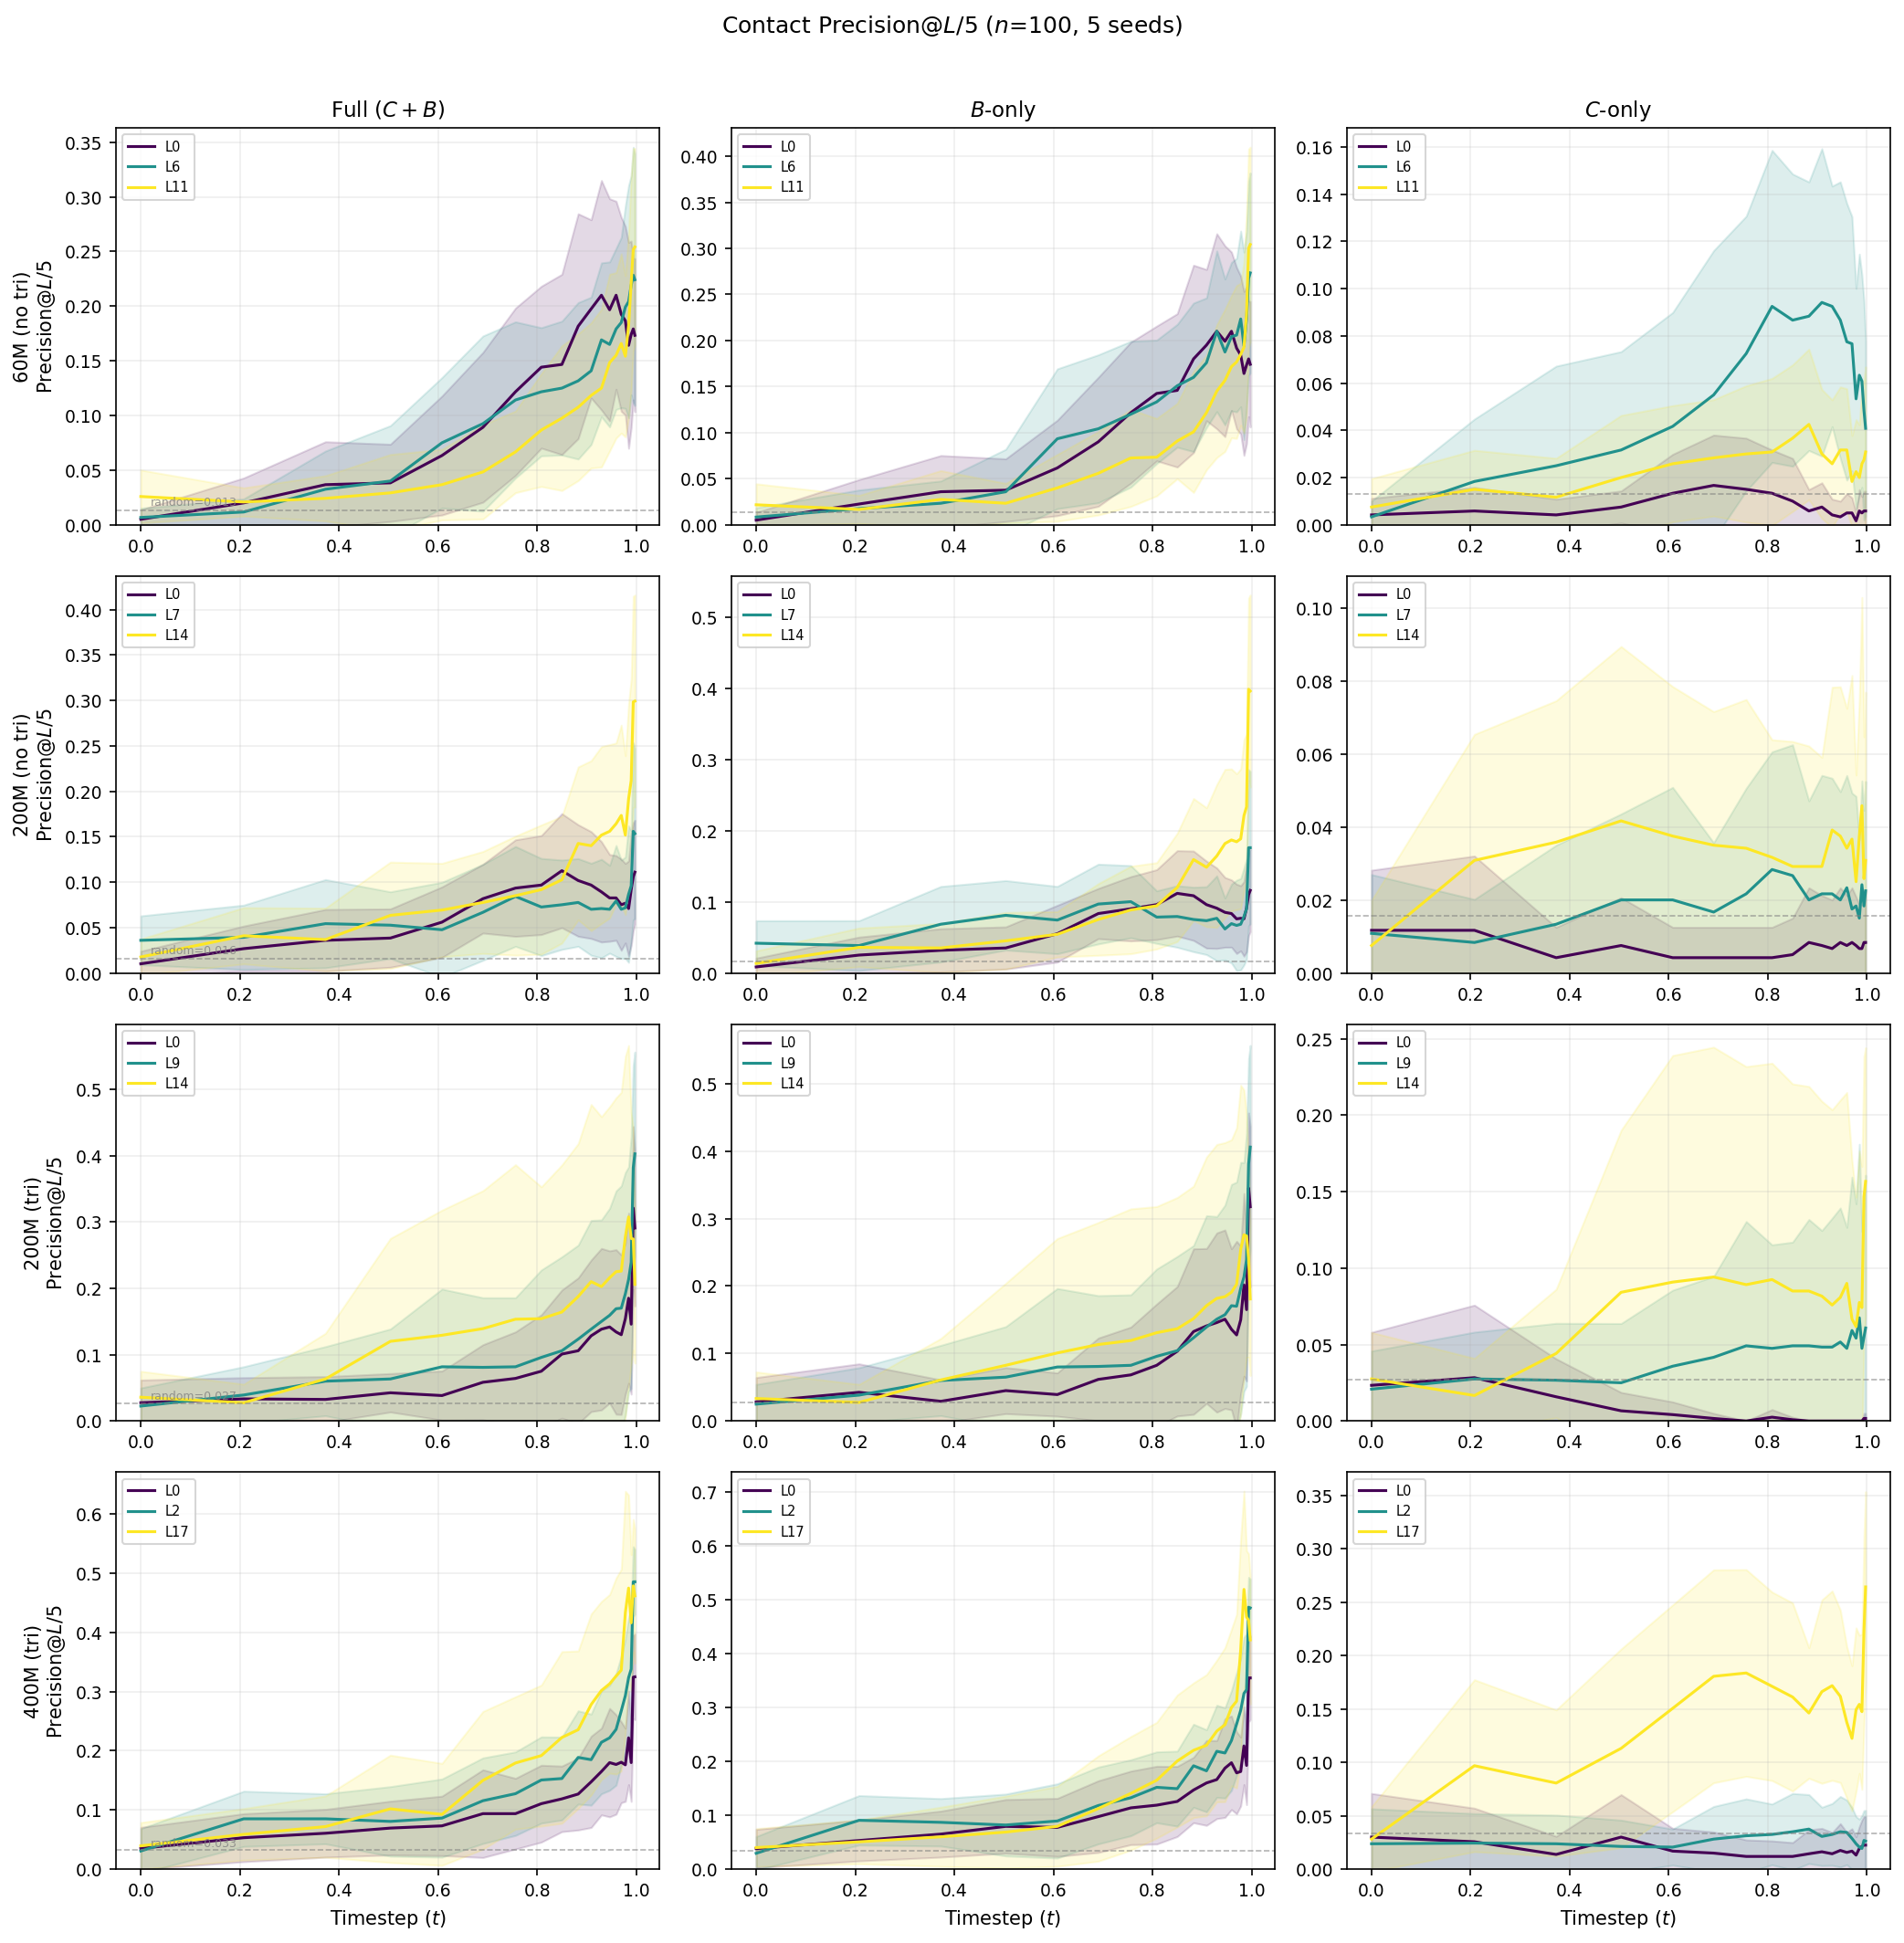
\includegraphics[width=\textwidth]{figures/fig3-contact-precision-all-models.png}
\end{figure}

\vspace{-0.5em}
{\small $B$-only attention encodes contacts; $C$-only never catches up.}

\end{column}
\begin{column}{0.48\textwidth}

\textbf{Structure Emerges Only at the Output}
\smallskip

\begin{figure}
    \centering
    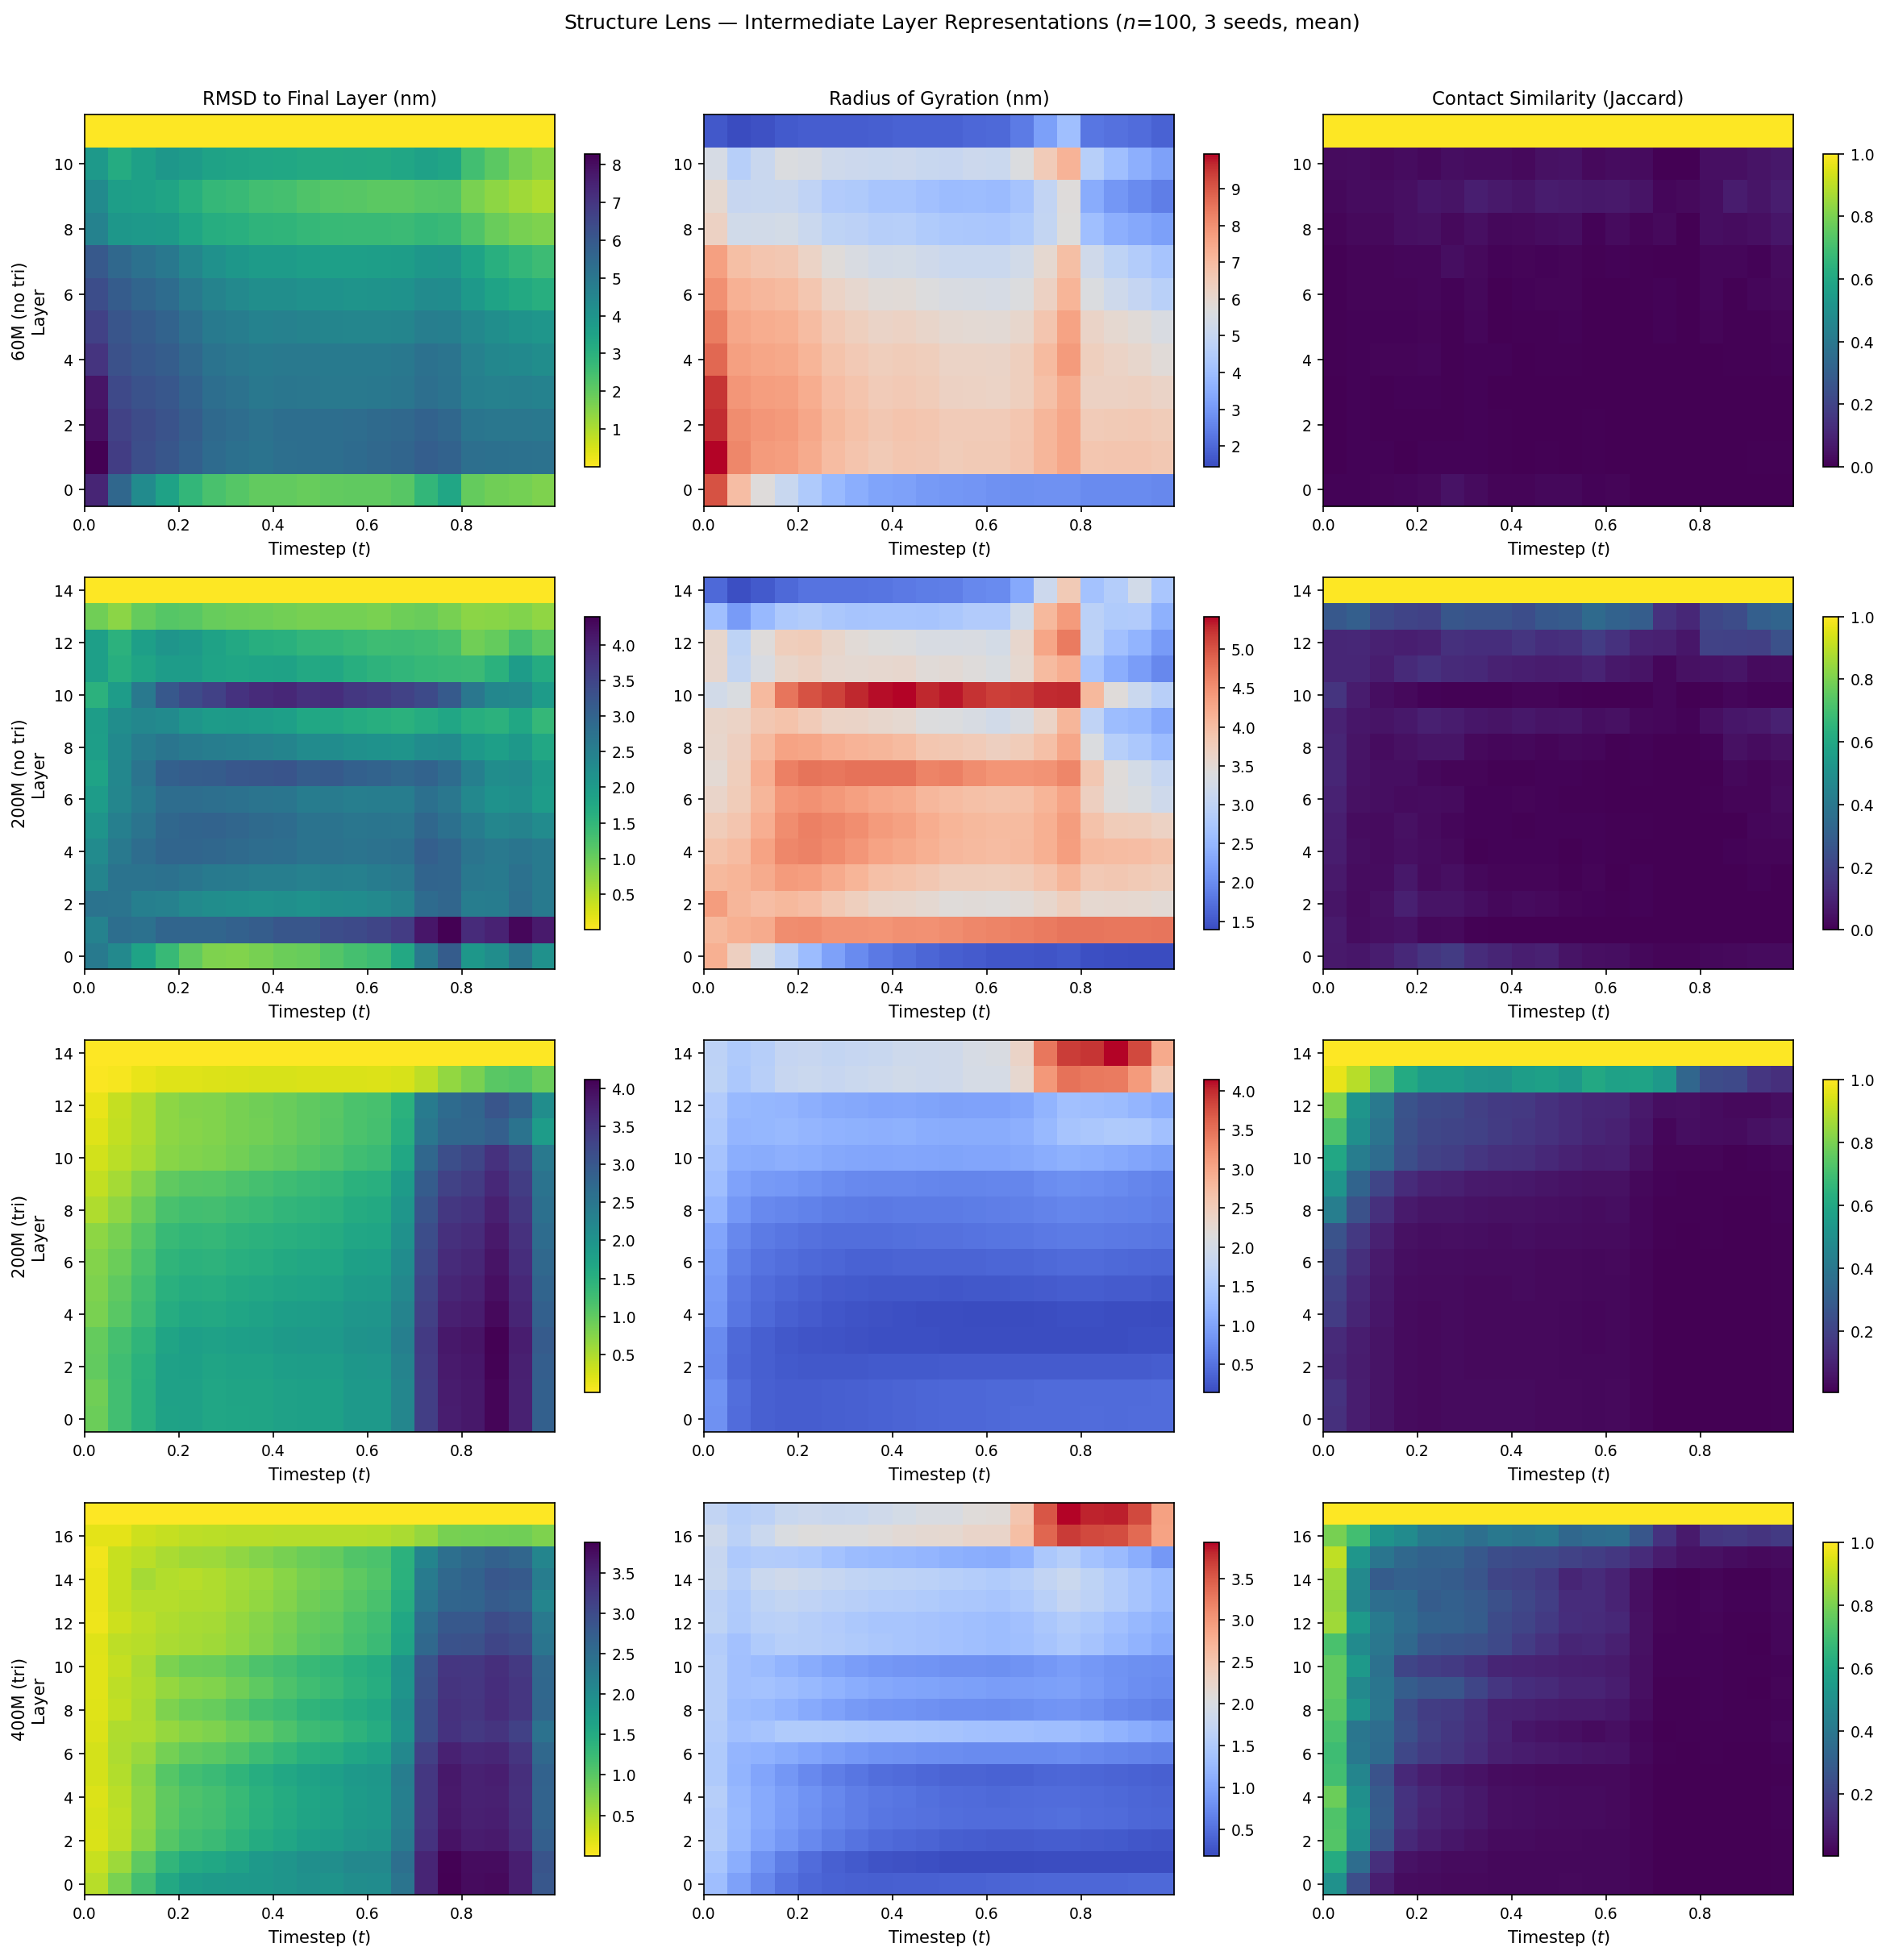
\includegraphics[width=\textwidth]{figures/fig5-structure-lens-all-models.png}
\end{figure}

\vspace{-0.5em}
{\small Contact similarity near zero until last 1--2 layers.}

\end{column}
\end{columns}
\end{frame}

% ============================================================
\begin{frame}{Summary}

\begin{block}{Finding 1: Geometric guidance is memoryless}
Only the \emph{present} matters. Early $B$ leaves no trace.
Late-only $B$ always preserves valid structures. Early-only $B \equiv$ no $B$.
\end{block}

\begin{block}{Finding 2: Architecture determines where, not when}
Triangle updates invert spatial sensitivity (shallow $\leftrightarrow$ deep),
but the temporal asymmetry is identical across all four model scales.
\end{block}

\begin{block}{Finding 3: Descriptive $\neq$ causal}
$R_c$ varies from 0.5 to 35 across models. Peak-$R_c$ layer is not the critical layer.
Multi-lens analysis is required to avoid misleading conclusions.
\end{block}

\end{frame}

% ============================================================
\begin{frame}{Implications \& Future Work}

\textbf{If $B$ is actionable only during late generation:}

\vfill

\begin{columns}[T]
\begin{column}{0.48\textwidth}
\begin{block}{Late-stage geometric steering}
Align intermediate representations to structure-based objectives (atomic potentials, fold classifiers) during the \textbf{final denoising steps only}.

Early steps can be left free.
\end{block}
\end{column}

\begin{column}{0.48\textwidth}
\begin{block}{Early-stage representation alignment}
If early $B$ is not used, early generation may benefit from \textbf{content-aligned objectives} (cf.\ REPA, Yu et al.\ 2025).

Connect flow models to representation alignment literature.
\end{block}
\end{column}
\end{columns}

\vfill

\centering
Code: \texttt{github.com/rs-gh/proteina-interpretability}

\end{frame}

\end{document}
